\section{Introduction}
\label{sec:introduction}

\IEEEPARstart{S}{imulation} of multibody systems with frictional contact has
proven indispensable in robotics, aiding at multiple stages during the
mechanical and control design, testing, and training of robotic systems. Robotic
applications often require robust simulation tools that can perform at
interactive rates without sacrificing accuracy, a critical prerequisite for
meaningful sim-to-real transfer. However, reliable modeling and simulation for
contact-rich robotic applications remains somewhat elusive.

Rigid body dynamics with frictional contact is complicated by the non-smooth
nature of the solutions. It is well known \cite{bib:baraff1993issues} that rigid
contact when combined with the Coulomb model of friction can lead to paradoxical
configurations for which solutions in terms of accelerations and forces do not
exist. These phenomena are known as Painlev\'e paradoxes
\cite{bib:hogan2017regularization}.
%
\begin{figure}[!ht]
	\centering
    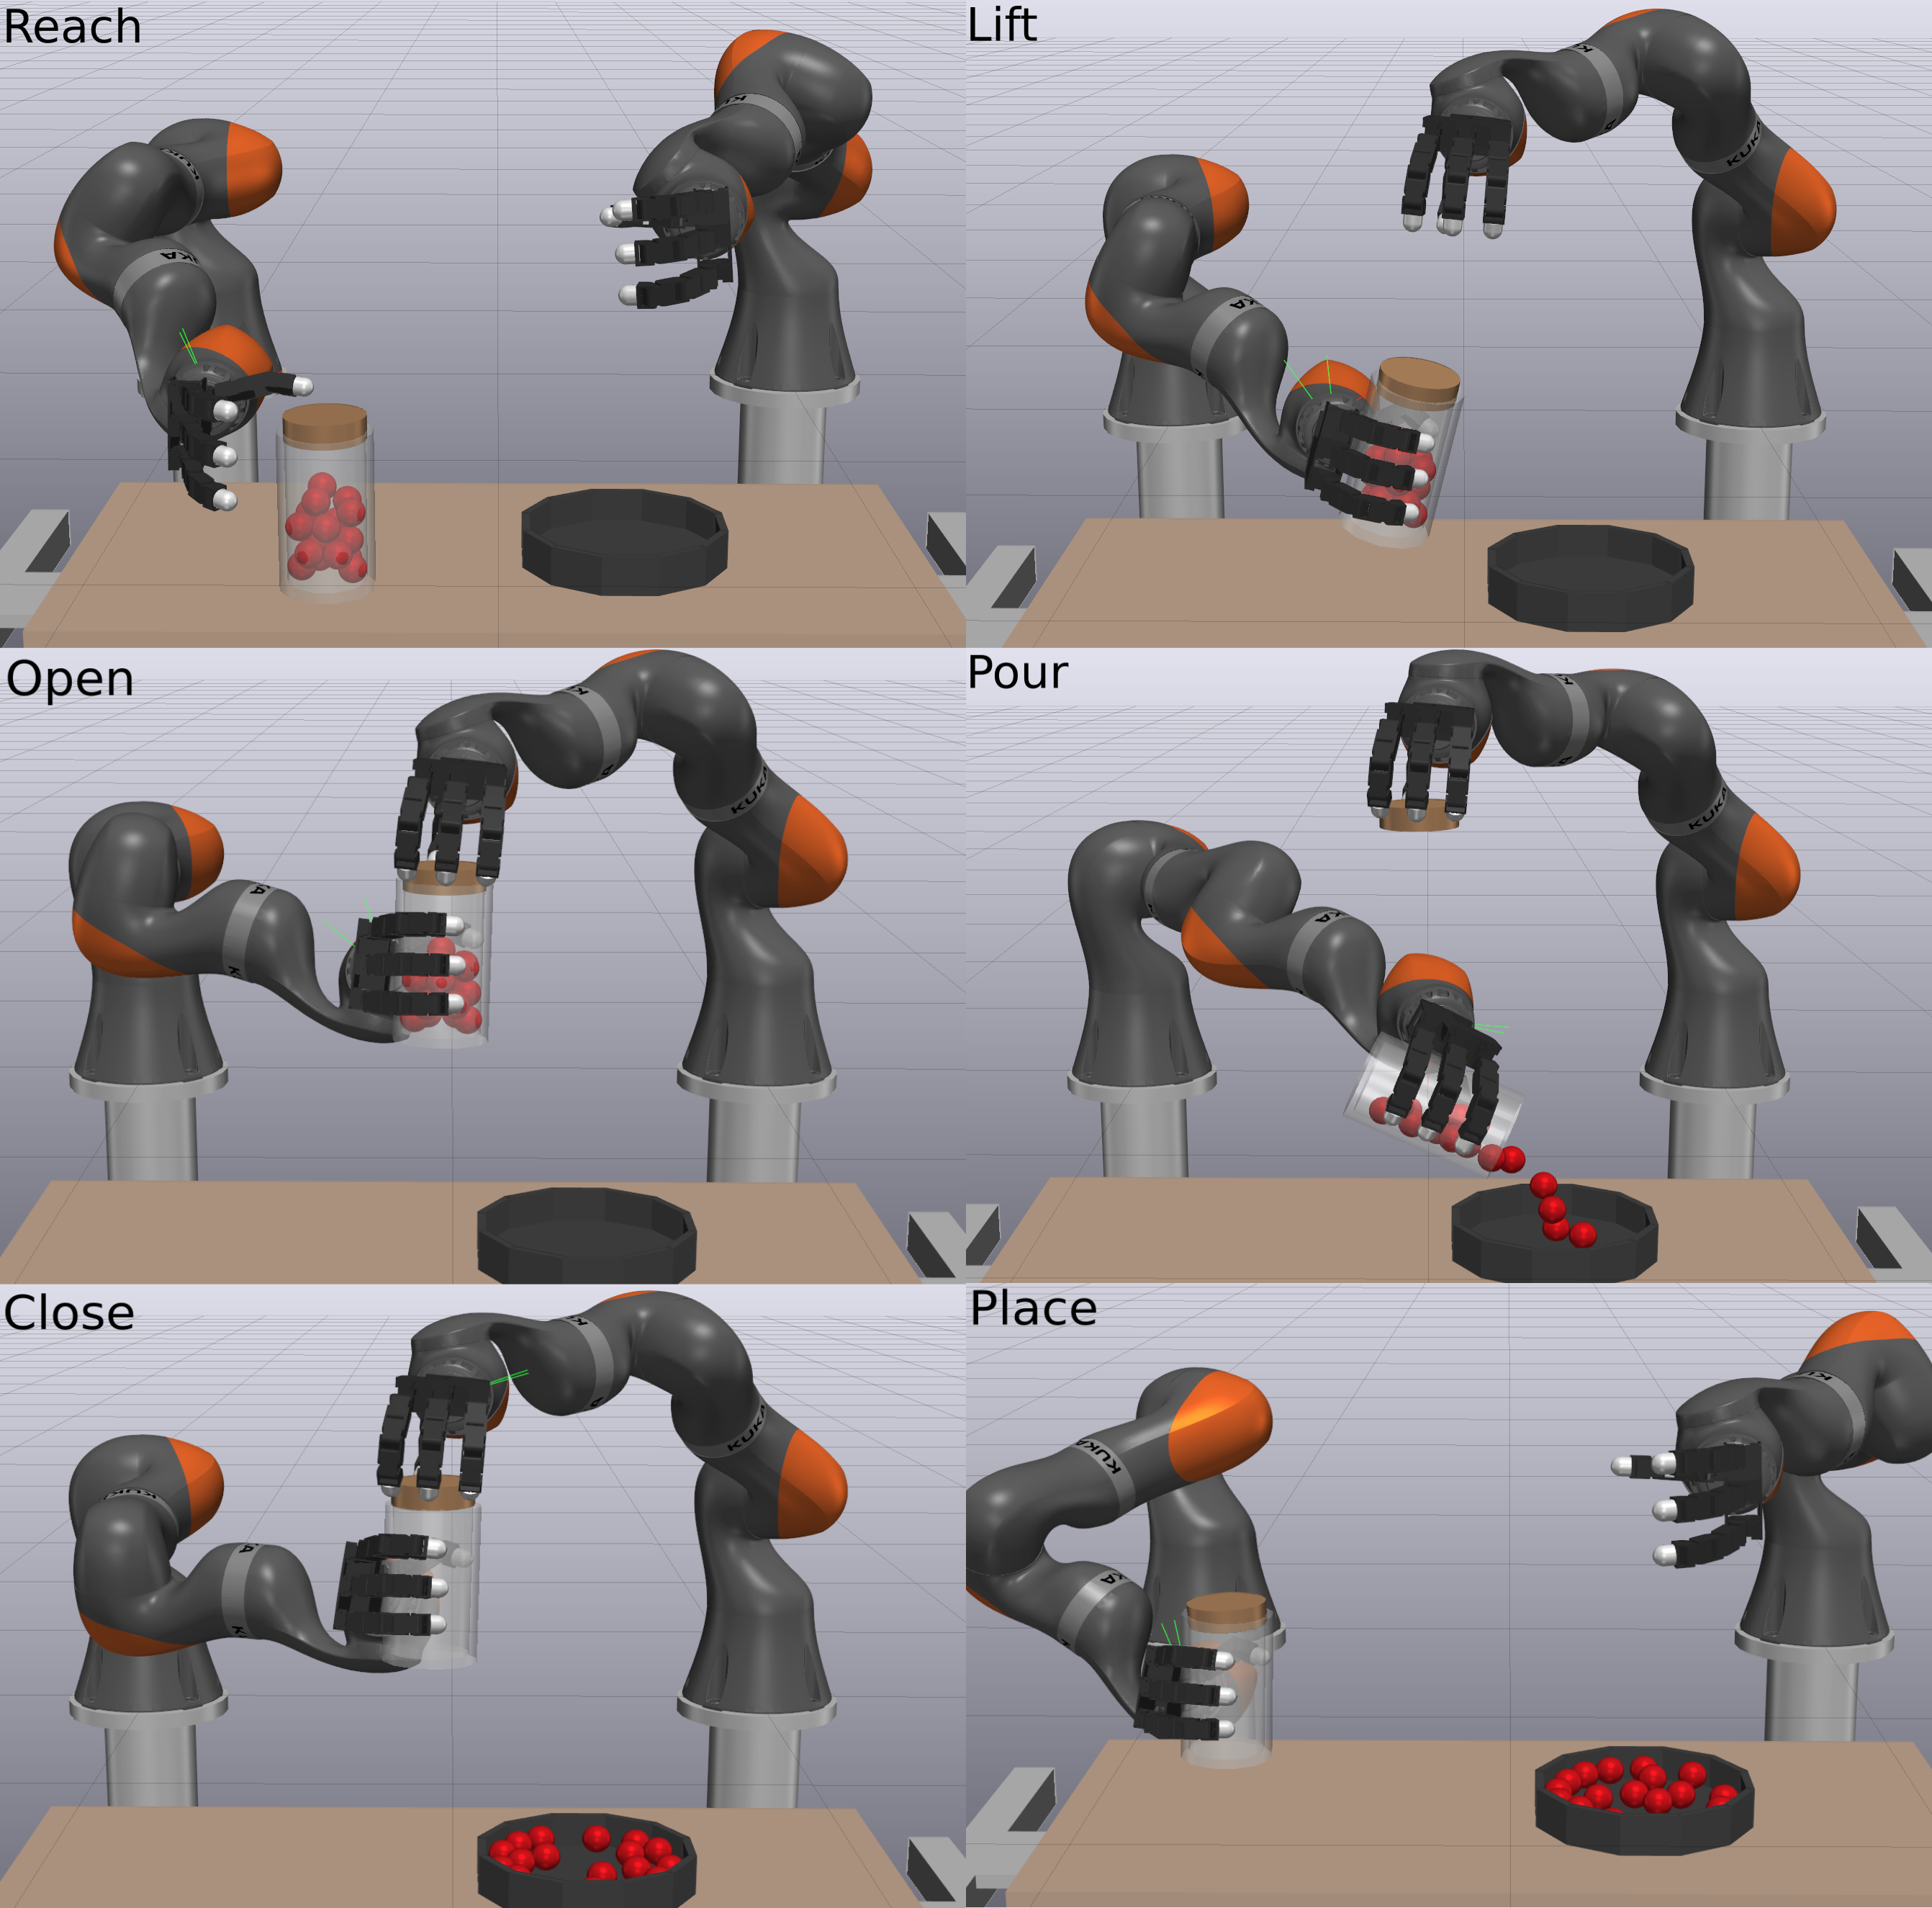
\includegraphics[width=0.95\columnwidth]{figures/dual_arm/tiled.png}
	\caption{\label{fig:dual_arm_frames}
    Keyframes of a dual arm manipulation task in simulation (see supplemental
    video). The robot is commanded to pick up a jar full of marbles, open it,
    pour its contents into a bowl, close the lid and place the empty jar back in
    place. This is a computationally intensive simulation with 160 degrees of
    freedom and hundreds of contact constraints per time step (see Fig.
    \ref{fig:dual_arm_contacts}). Our SAP solver is robust and warm-starts
    effectively, enabling this simulation to run at interactive rates.}
\end{figure}
%
Theory resolves these paradoxes by allowing discrete velocity jumps and
impulsive forces, formally casting the problem as a differential variational
inequality \cite{bib:pang2008differential}. In practice, event based approaches
can resolve impulsive transitions \cite{bib:haug1986}, though it is not clear
how to reliably detect these events even for simple one degree of freedom
systems \cite{bib:hogan2017regularization}.

Nevertheless, the problem can be solved in a weaker formulation at the velocity
level using a time-stepping scheme where the next step velocities and impulses
are the unknowns at each time step \cite{bib:stewart1996implicit,
bib:anitescu1997}. These formulations lead in general to a non-linear
complementarity problem (NCP). A linear complementarity problem (LCP) can be
formulated using a polyhedral approximation of friction cones, though at the
expense of non-physical anisotropy \cite{bib:li2018implicit}. Even though LCP
formulations guarantee solution existence \cite{bib:anitescu1997,
bib:stewart1998convergence}, solving them accurately and efficiently has
remained difficult in practice. This has been explained partly due to the fact
that these formulations are equivalent to nonconvex problems in global
optimization, which are generally NP-hard \cite{bib:Kaufman2008}. Indeed,
popular direct methods based on Lemke's pivoting algorithm to solve LCPs may
exhibit exponential worst-case complexity \cite{bib:baraff1994fast}. Similarly,
popular iterative methods based on projected Gauss-Seidel (PGS)
\cite{bib:duriez2006_realistic_haptic_rendering, bib:bullet} have also shown
exponentially slow convergence \cite{bib:erleben2007velocity}. These
observations are not just of theoretical value---in practice, these methods are
numerically brittle and lack robustness when tasked with computing contact
forces. Software typically attempts to compensate for this inherent lack of
stability and robustness through non-physical constraint relaxation and
stabilization, requiring a significant amount of application-specific parameter
tuning.

\subsection{Previous Work on Convex Approximations of Contact}
To improve computational tractability, Anitescu introduced a \textit{convex
relaxation} of the contact problem \cite{bib:anitescu2006}. This relaxation is a
convex approximation with proven convergence to the solution of a measure
differential inclusion as the time step goes to zero. \reviewquestion{R4-Q1}{For
sliding contacts, the convex approximation introduces a \emph{gliding} artifact
at a distance $\phi$ that is proportional to the time step $\delta t$, friction
coefficient $\mu$ and sliding velocity $\Vert\vf{v}_t\Vert$
\cite{bib:mazhar2014}, i.e. $\phi\sim \delta t\mu\Vert\vf{v}_t\Vert$. This
artifact can be irrelevant for problems with lubricated contacts (as in many
mechanisms) and goes away for sticking contacts (dominant in robotic
manipulation). For sliding contact, the approximation can be adequate for
applications for which the product $\delta t\mu\Vert\vf{v}_t\Vert$ is usually
sufficiently small.} For trajectory optimization, Todorov \cite{bib:todorov2011}
introduces regularization into Anitescu's formulation in order to write a
strictly convex formulation with a unique, smooth and invertible solution. For
simulation, Todorov \cite{bib:todorov2014} uses regularization to introduce
\emph{numerical compliance} that provides Baumgarte-like stabilization to avoid
constraint drift. As a side effect, the regularized formulation can lead to a
noticeable non-zero slip velocity even during stiction \cite{bib:simbenchmark}.

\subsection{Available Software}
Even though these formulations introduce a tractable approximation of frictional
contact, they have not been widely adopted in practice. We believe this is
because of the lack of robust solution methods with a computational cost
suitable for interactive simulation. Software such as ODE \cite{bib:ode}, Dart
\cite{bib:dart} and Vortex \cite{bib:vortex} use a polyhedral approximation of
the friction cone leading to an LCP formulation. Algoryx \cite{bib:algoryx} uses
a \emph{split solver}, reminiscent of one iteration in the staggered projections
method \cite{bib:Kaufman2008}. \reviewquestion{AE-Q3}{RaiSim \cite{bib:raisim}
implements an iterative method with exact solution per-contact, a significant
improvement over the popular PGS used in computer graphics, though still
with no convergence nor accuracy guarantees.} Drake \cite{bib:drake} solves
compliant contact with regularized friction with its transition aware solver
TAMSI \cite{bib:castro2020}.

To our knowledge, Chrono \cite{bib:chrono2016}, Mujoco \cite{bib:mujoco} and
Siconos \cite{bib:acary2019siconos} are the only packages that implement the
convex approximation of contact. \reviewquestion{R4-Q2}{Chrono implements a
variety of solvers for Anitescu's convex formulation \cite{bib:anitescu2006}
including projected Jacobi and Gauss-Seidel methods \cite{bib:tasora2011},
Accelerated Projected Gradient Descent (APGD) \cite{bib:mazhar2015}, Spectral
Projected Gradients (SPG) \cite{bib:heyn2013using} and more recently Alternating
Direction Method of Multipliers (ADMM) \cite{bib:tasora2021solving}. Though
these methods are first order and often exhibit slow convergence, they are
amenable to parallelization and have been applied successfully in the simulation
of granular flows with millions of bodies.} MuJoCo targets robotic applications.
It's contact model is parameterized by a daunting number of non-physical
parameters aimed at regularizing the problem, though at the expense of drift
artifacts \cite{bib:simbenchmark}. Still, it has become very popular in the
reinforcement learning community given its performance.
\reviewquestion{R1-Q8}{Siconos is an open-source software targeting
large scale simulation of both rigid and deformable objects. The authors of
Siconos perform an exhaustive benchmarking campaign in
\cite{bib:acary2018solving} using the convex approximation of contact. The
analysis reveals that there is no universal solver and that every solver
technology suffers from accuracy, robustness and/or efficiency problems.}

\subsection{Outline and Novel Contributions}
\reviewquestion{R1-Q9}{It is not even clear if these convex approximations
present a real advantage when compared to approaches solving the original
non-convex NCP problem and whether the artifacts introduced by the approximation
are acceptable for robotics applications.} In this work, we propose a new
unconstrained convex approximation and discuss techniques for its efficient
implementation. We carefully quantify the artifacts introduced by the convex
approximation and evaluate the robustness and accuracy of our method on a family
of examples.

We introduce a two-stage time stepping approach (Section
\ref{sec:discrete_time_formulation}) that allows us to incorporate both first
and second order schemes such as the midpoit rule. In Section \ref{sec:spring_cylinder} we
demonstrate that the midpoint rule can achieve second order accuracy even in
problems with frictional contact. Unlike previous work
\cite{bib:anitescu2010,bib:todorov2014} that formulates the problem in its dual
form (impulses), we write a primal formulation of compliant contact in
velocities (Section \ref{sec:primal_formulation}). We then analytically
eliminate constraints from this formulation to obtain an unconstrained convex
problem (Section \ref{sec:unconstrained_convex_formulation}).

To solve this formulation, we develop SAP---the Semi-Analytic Primal solver---in
Section \ref{sec:sap_solver} and study its theoretical and practical
convergence.  Crucially, we show that SAP globally converges from all initial
conditions (Appendix \ref{app:sap_converge}) and warm-starts effectively using
the previous time-step velocities, enabling simulation at interactive rates.

To address accuracy and model validity,
Section \ref{sec:physical_intuition} provides compact analytic formulae for the
impulses that correspond to the optimal velocities of the convex approximation.
This provides intuition for the approximation, even to those without
optimization expertise. Moreover, the artifacts introduced by the approximation
become apparent and can be characterized precisely. \reviewquestion{AE-Q7}{We
provide an exact mapping between the regularization introduced by Todorov
\cite{bib:todorov2014} to \emph{physical} parameters of compliance. Therefore
regularization is no longer treated as a tuning parameter of the algorithm but
as a true physical parameterization of the contact model. This allows us to
incorporate not only compliant point contact, but also complex models of
compliant surface patches \cite{bib:elandt2019pressure,
bib:masterjohn2021discrete}, as we demonstrate in Section
\ref{sec:slip_control}.}

We demonstrate the effectiveness of our approach in Section \ref{sec:test_cases}
in a number of simulation cases, including the simulation of the challenging
dual arm manipulation task shown in Fig. \ref{fig:dual_arm_frames}. We evaluate
the accuracy, robustness and performance of SAP against available commercial and
open-source optimization solvers.

Finally, we discuss extensions and variations in Section
\ref{sec:variations_and_extensions}, limitations in Section
\ref{sec:limitations} and conclude with final remarks in Section
\ref{sec:future_directions}.
